\chapter{Zanarkand}
\begin{enumerate}
	\item \sd, \cs[0:50], walk left. \fmv+\cs[2:20]
	\item Move left to the sphere, \sd, \cs[1:40]. Walk further left and follow the path down, \cs[3:20], walk left onto the next screen.
	\item \formation{\tidus}{\auron}{\kimahri} \textit{if you don't need to build \rikku\ \od\ else} \formation{\tidus}{\auron}{\rikku}.
	\item Make sure to build \rikku\ \od\ on Behemoth or Defender Z, unless you want to use a Skill Sphere on the Final Boss for Armor Break.
	\item If you missed the Overkill on \textbf{Seymour Flux}, then kill two \textbf{YKT-11} or one \textbf{Defender Z} with \yuna\ and \tidus, with \formation{\tidus}{\yuna}{\auron}. Only \yuna\ needs the AP.
\end{enumerate}
\begin{encounters}
	\begin{itemize}
		\item YKT-11:
		      \begin{itemize}
			      \tidusf Attack
			      \yunaf Attack
		      \end{itemize}
		\item Singular Defender Z Inside of Dome:
		      \begin{itemize}
			      \summon{\bahamut}
			      \bahamutf Attack
		      \end{itemize}
	\end{itemize}
\end{encounters}
\begin{enumerate}[resume]
	\item Continue on the path. \pickup{Fortune Sphere} on the left of the road. Seymour's Mom \cs
	\item After the \cs, \pickup{Friend Sphere} on the right, \textbf{skip} it if you had 0 or 2 Return Spheres. When you leave the last encounter zone, the hallway before the Zanarkand Trials, \pickup{Luck Sphere} on the right.
\end{enumerate}
\bothvfill
\bothnp
\winvfill
\winnp
\lossvfill
\lossnp
\begin{spheregrid}
	\begin{itemize}
		\yunaf
		\begin{itemize}
			\item \textit{If you got \textbf{4 Return Spheres}:}
			      \begin{itemize}
				      \item Friend Sphere to \lulu $\downarrow\downarrow$
				      \item Luck Sphere, Fortune Sphere
				      \item Str+4, Str+4
				      \item Move $\nearrow\uparrow\uparrow$
				      \item Agi+4, Agi+4, Str+3
			      \end{itemize}
			      \ifthenelse{\equal{\colstyle}{multi}}{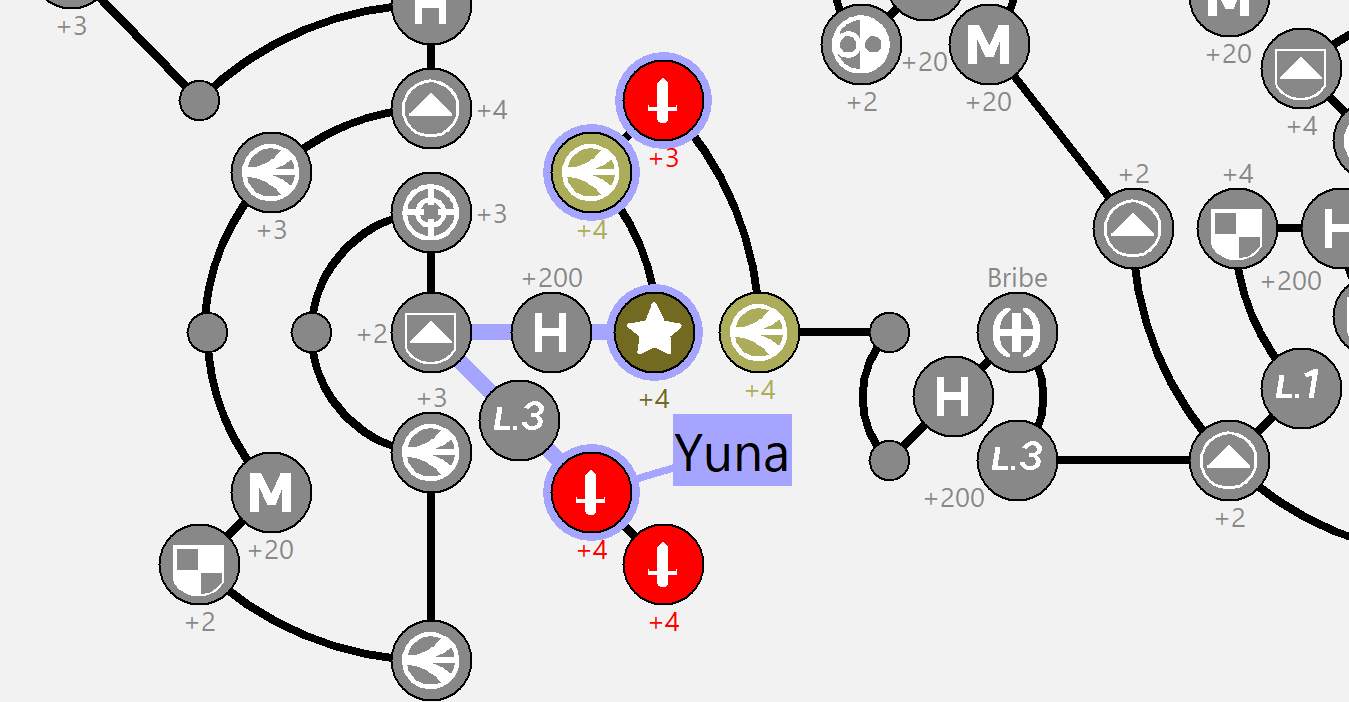
\includegraphics[width=.5\columnwidth]{graphics/4_returns_w_luck_pt1}}{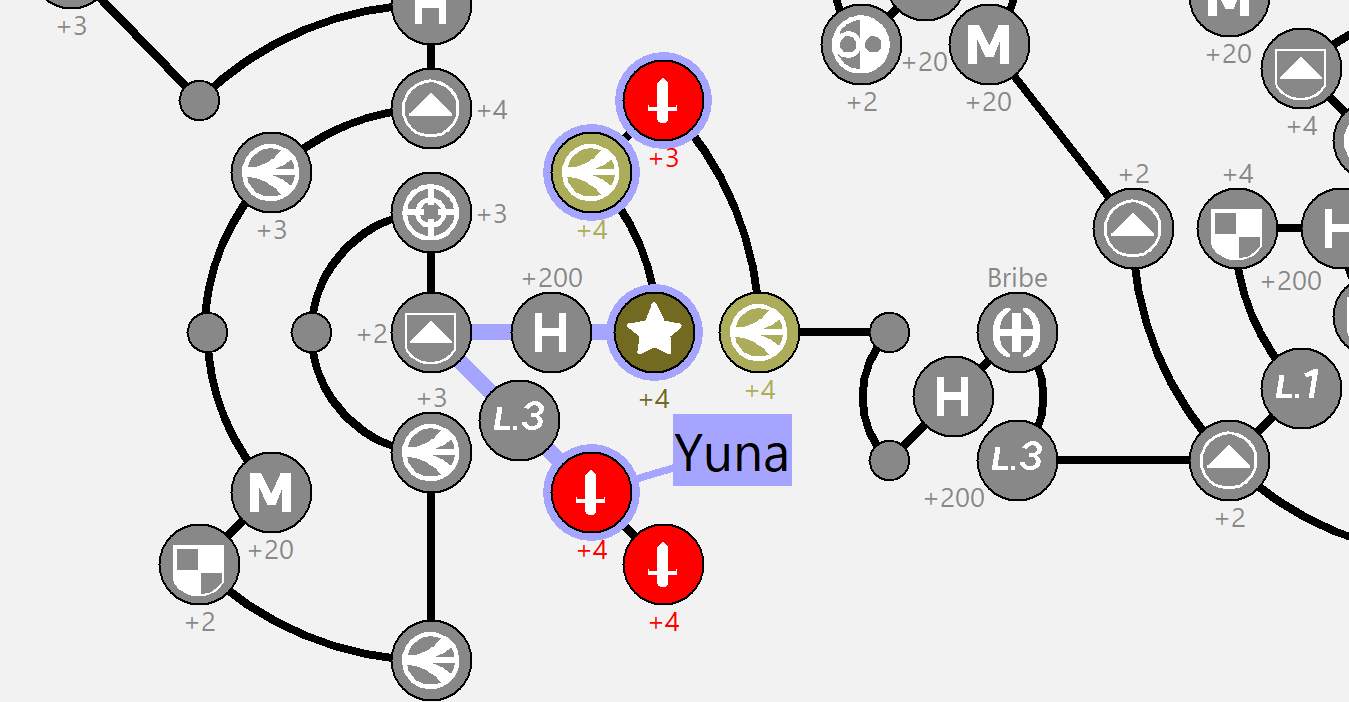
\includegraphics[width=.2\columnwidth]{graphics/4_returns_w_luck_pt1}}
			\item \textit{If you got \textbf{2 Return Spheres}:}
			      \begin{itemize}
				      \item Return Sphere to Str+2 in \wakka's grid, $\nearrow$
				      \item Move $\leftarrow$
				      \item Level 1 Key Sphere, Mag+3
				      \item Luck Sphere, Fortune Sphere
				      \item Move $\searrow\searrow$
				      \item Agi+4, Str+2
				      \item Move $\leftarrow\leftarrow$
				      \item Agi+3, Str+2
				      \item Move $\downarrow$
				      \item Str+2
			      \end{itemize}
			      \ifthenelse{\equal{\colstyle}{multi}}{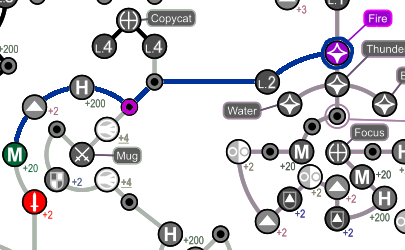
\includegraphics[width=.5\columnwidth]{graphics/2_and_2_with_luck}}{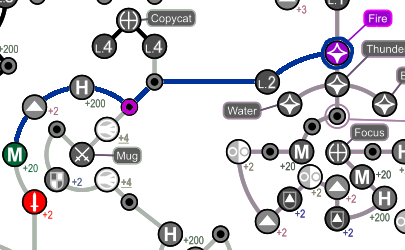
\includegraphics[width=.2\columnwidth]{graphics/2_and_2_with_luck}}
			\item \textit{If you got \textbf{0 Return Spheres}:}
			      \begin{itemize}
				      \item Move $\downarrow\downarrow$
				      \item Luck Sphere, Fortune Sphere
			      \end{itemize}
			      \ifthenelse{\equal{\colstyle}{multi}}{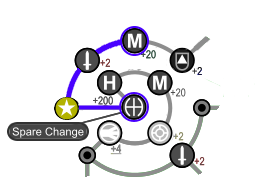
\includegraphics[width=.7\columnwidth]{graphics/0_return_w_luck}}{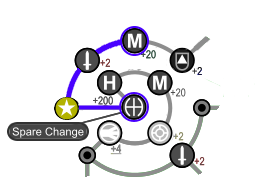
\includegraphics[width=.25\columnwidth]{graphics/0_return_w_luck}}
		\end{itemize}
	\end{itemize}
\end{spheregrid}
\bothcb \wincb \losscb
\begin{enumerate}[resume]
	\item \formation{\tidus}{\auron}{\yuna}
	\item \textit{If you had 0 Return Spheres:}
	      \begin{itemize}
		      \item Customize:
		            \begin{itemize}
			            \auronf Shimmering Blade $\rightarrow$ First Strike
			            \yunaf Staff $\rightarrow$ First Strike
		            \end{itemize}
	      \end{itemize}
\end{enumerate}
\begin{equip}
	\begin{itemize}
		\item Auron: Sonic Blade
	\end{itemize}
\end{equip}
\begin{enumerate}[resume]
	\item {\large \save}
\end{enumerate}
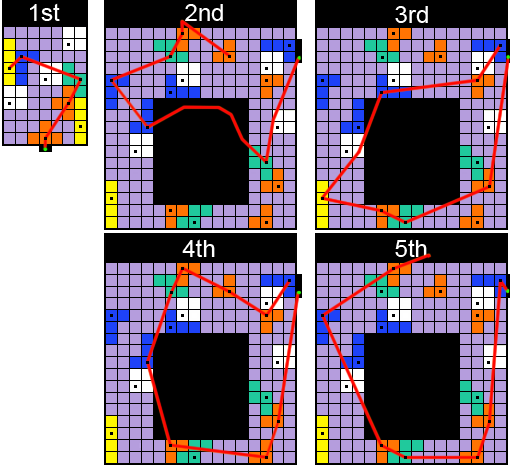
\includegraphics[width=.95\columnwidth]{graphics/Zanarkand_Trials}
\begin{enumerate}[resume]
	\item Push in the pedestals starting from the Top Left, to Bottom Left, then Top Right, Bottom Right, then Besaid Sphere. After pushing in each pedestal, do the corresponding puzzle, shown above.
	\item After the second puzzle, take the Kilika Sphere on the left and put it into the second pedestal.
	\item After the fifth puzzle, take the Besaid Sphere from the right and put it into the fifth pedestal.
	\item \cs, run into the large room
\end{enumerate}
\begin{battle}[52000]{Spectral Keeper}
	\begin{itemize}
		\summon{\bahamut}
		\bahamutf Attack
	\end{itemize}
\end{battle}
\bothvfill\winvfill\lossvfill
\begin{spheregrid}
	\begin{itemize}
		\item \textit{If you had 4 \textbf{Return Spheres}}:
		      \begin{itemize}
			      \item Return Sphere to Mag+3 in \wakka's Grid, $\uparrow\rightarrow\downarrow$ or $\nearrow$
			      \item Move $\rightarrow$
			      \item Str+2
			      \item Move $\downarrow\downarrow$
			      \item Str+2, Agi+3
		      \end{itemize}
		\item \yuna\ should have 70 Str and 35 Agi. If short, then the key Str Nodes are near \tidus's Armor Break and the end of \wakka's grid, and Agi is near \lulu\ (+8), \rikku\ (+3) and \wakka (+3 near Mag+3). If you need more Return Spheres to do these, then you can attack Sinspawn Genais for an extra one, though it costs 26 seconds
	\end{itemize}
	\ifthenelse{\equal{\colstyle}{multi}}{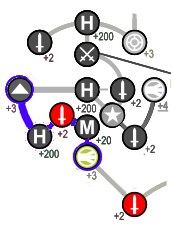
\includegraphics[width=.5\columnwidth]{graphics/4_return_before_yunalesca}}{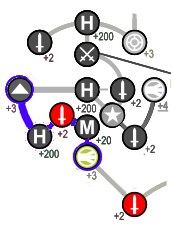
\includegraphics[width=.25\columnwidth]{graphics/4_return_before_yunalesca}}
\end{spheregrid}
\begin{enumerate}[resume]
	\item \save, Run up, \sd by mashing another button (like \textbf{R1}) at the same time as confirm, walk up to Yunalesca's room, \sd
\end{enumerate}
\begin{battle}[132000]{Yunalesca}
	\begin{itemize}
		\summon{\bahamut}
		\bahamutf Attack
	\end{itemize}
	Check for any weapon drops with \textbf{Zombie Strike}
\end{battle}
\begin{enumerate}[resume]
	\item \sd, leave room, walk down steps, \sd, go down on the next screens, \save, go up the lift, walk out of the cloister of trials, walk down the steps, walk down, \sd\ during \cs+\skippablefmv
\end{enumerate}